% Paper 6 (T6) -- IEEE JBHI special issue "Integrating Imaging with Personalized Cardiovascular Medicine"
% Deadline 2026-10-15. Target: 8 pages (over-length charges start at page 9).
% Plan and word budgets: BENCHMARK-AND-PLAN-JBHI-2026-10-03.md
\documentclass[journal]{IEEEtran}
\usepackage{amsmath,amssymb}
\usepackage{graphicx}
\usepackage{booktabs}
\usepackage{siunitx}
\usepackage[hidelinks]{hyperref}

\renewcommand{\dbltopfraction}{0.9}\renewcommand{\topfraction}{0.9}\renewcommand{\textfraction}{0.07}
\begin{document}
\bstctlcite{IEEEexample:BSTcontrol}

\title{Topological Segmentation Error and Boundary-Condition Tuning in Computed Coronary FFR: A Controlled In
Silico Study}
% Working title; alternative from STUDY-PLAN-v2 sec. 0:
% "Matched at the Outlet, Wrong in the Tree: ..."

\author{Fadillah~Yamin,
        Mohd~Azan~Mohammed~Sapardi,
        Ming~Kwang~Tan,
        Xin~Wang,
        and~Mohd-Zulhilmi~Paiz~Ismadi%
\thanks{F. Yamin, X. Wang and M.-Z. P. Ismadi are with the Department of Mechanical Engineering, School of
Engineering, Monash University Malaysia, 47500 Bandar Sunway, Selangor, Malaysia (corresponding author:
M.-Z. P. Ismadi, e-mail: mohd.zulhilmi@monash.edu).}%
\thanks{M. A. Mohammed Sapardi is with the Department of Mechanical Engineering, Kulliyyah of Engineering,
International Islamic University Malaysia, 53100 Kuala Lumpur, Malaysia.}%
\thanks{M. K. Tan is with the Department of Mechanical Engineering, School of Engineering, Monash University
Malaysia, and the Department of Mechanical Engineering, Ming Chi University of Technology, New Taipei City 243,
Taiwan.}}

\markboth{IEEE Journal of Biomedical and Health Informatics}{Yamin \MakeLowercase{\textit{et al.}}: Segmentation Error and BC Tuning in Coronary FFR}

\maketitle

\begin{abstract}
Fractional flow reserve, the pressure ratio that decides whether a coronary narrowing is treated, can be computed
from computed tomography angiography. The computation depends on the segmented artery and on outlet boundary
conditions derived from it, often tuned to match measured perfusion. Whether a model that matches perfusion can
still assign the wrong treatment at 0.80 has not been tested. We inserted 150 stenoses into 108 coronary trees,
applied four segmentation error types (missed side branch, vessel break, longer lesion, narrowed taper), and
recomputed fractional flow reserve with a reduced-order model under fixed, re-derived and perfusion-tuned boundary
conditions, with one global or one per-territory tuning parameter, in two microvascular bed structures. With fixed boundary conditions, branching (topological) errors changed the decision in
32--33\% of models, against 6--10\% for vessel-size (caliber) errors of inter-observer magnitude. Re-derived or tuned
boundary conditions reduced topological decision changes to 5--19\%. Tuning matched perfusion but did not remove
every error: 5--20\% of tuned topological-error models and 4--18\% of tuned caliber-error models passed a perfusion
check stricter than measurement repeatability while wrong by more than 0.05, against 3--4\% for correct anatomy and
none for caliber errors with re-derived boundary conditions. Per-territory tuning corrected the typical missed
branch; in three dimensions it reduced a shift of 0.074 to $-0.0007$, as the reduced-order model predicted. The
directions held at doubled and tripled hyperemic demand. A perfusion match after tuning therefore does not show that
the computed value is correct; branching and caliber must be checked before tuning.
\end{abstract}

\begin{IEEEkeywords}
Boundary conditions, coronary artery disease, fractional flow reserve, image segmentation, reduced-order modeling,
uncertainty.
\end{IEEEkeywords}

% ---------------------------------------------------------------------------------------------------------------
\section{Introduction}
\IEEEPARstart{F}{ractional} flow reserve (FFR) is the pressure ratio that decides whether a coronary narrowing is treated. It is the blood pressure beyond the narrowing divided by the aortic pressure during maximal flow. A value at or
below 0.80 marks a stenosis for revascularization \cite{tonino2009}. FFR can also be computed without a pressure
wire. The lumen, the blood-filled channel of the artery, is segmented from coronary computed tomography (CT)
angiography and converted into a flow model, and the computed FFR has been validated against invasive measurement
in multicenter trials \cite{taylor2013,norgaard2014}. The calculation exists in three-dimensional (3D),
reduced-order and machine-learning forms \cite{kim2010,fossan2026,itu2016}.

Every such model needs boundary conditions, the pressures, flows or resistances imposed where the model ends to stand in for the vessels the image cannot resolve. The largest part of this unresolved circulation is the
microvascular bed, the arterioles and capillaries downstream of the segmented arteries, which set how much blood
each region of heart muscle draws. Its resistance is not measured but derived from the segmented lumen through
scaling laws that relate vessel size to the flow it carries \cite{murray1926,kim2010}. It is increasingly tuned so that the model reproduces measured perfusion, the blood flow to each region of heart
muscle, or measured flow splits \cite{menon2024,arminio2026}. The segmentation therefore enters the computed FFR twice, through the arteries and through the boundary conditions derived from them.

Segmentation error has been studied mainly as caliber error. Caliber is the inner diameter of a vessel, so a caliber error is a lumen drawn too wide or too narrow, or a narrowing drawn too long, while the branching is unchanged. Sensitivity analyses perturb the radius at fixed bifurcations and report a continuous change in the computed pressure index \cite{sankaran2015tmi,sankaran2015cmame,fernandez2024,dalmaso2025}. Studies that set geometry against
boundary conditions rank the two by their influence on a continuous output \cite{sankaran2016,tanade2022,korte2023}. Topological error, a change in the branching structure itself such as a missed side branch or a vessel that ends too early, has received less attention. In a pulmonary network model, connectivity contributed more to hemodynamic uncertainty than vessel radius and
length \cite{colebank2019}, and examples from a recent coronary benchmark showed vessel breaks in the output of every evaluated method despite high overlap scores \cite{bransby2026}, and small distal segments remain the hardest to segment
\cite{chen2025}. A missed branch removes part of the microvascular bed from the model and changes both the flow
through the stenosis and the boundary conditions derived from the tree.

Whether such an error reaches the computed FFR depends on how the boundary conditions are handled. With outlet resistance held fixed, adding a side branch beyond a stenosis lowered FFR by 15.5\% in an idealized model and by 13\% in one of two models built from optical coherence tomography \cite{gamage2022}. When a cohort-wide outlet resistance was recalibrated for a model with side-branch outflow, diagnostic accuracy changed little \cite{gosling2020}. In a clinical cohort, a change of outlet model moved sensitivity from 58.1\% to 68.6\% at an unchanged area under
the curve \cite{fossan2026}. If the boundary conditions are tuned until the model matches measured perfusion, a topological error may vanish
from the perfusion check yet remain in the pressure along the vessel. None of these studies compares fixed, re-derived and tuned boundary conditions on the same corrupted anatomy at
0.80, or tests whether a model can pass a perfusion check and still assign the wrong treatment.

We propose a controlled test for this problem, an ablation in which one segmentation error at a time is introduced
into an otherwise correct model, whose FFR serves as the true value, so every change in FFR can be traced to the error
and to the handling of the boundary conditions. The approach is new in three respects. First, segmentation error is judged by whether it changes the treatment
decision at 0.80, not by a continuous sensitivity, and against the variability of repeat invasive FFR. Second, the
same corrupted anatomy is solved under fixed, re-derived and tuned boundary conditions, with tuning by one global or
one per-territory parameter, which isolates the effect of tuning, and topological errors are separated from caliber
errors of measured inter-observer magnitude. Third, the test counts how often a model passes a perfusion check while
its FFR is materially wrong, a failure of the check that, to our knowledge, has not been quantified, and a 3D
computational fluid dynamics (CFD) case tests the reduced-order result. The results show what a perfusion check
misses and which further checks a computed-FFR pipeline needs.

% ---------------------------------------------------------------------------------------------------------------
\section{Methods}
\begin{figure*}[!t]\centering
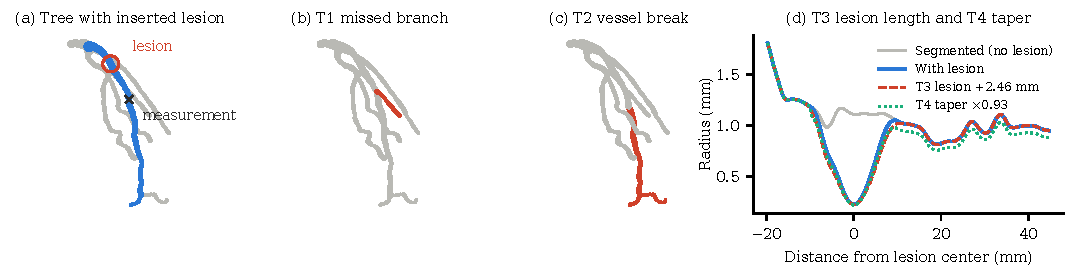
\includegraphics[width=\textwidth]{figures/fig1_errors.pdf}
\caption{The four segmentation error types on one cohort tree (left coronary tree of scan 14, front view, line width
proportional to radius). (a) The tree with an inserted 80\% DS lesion in the proximal LAD (blue) and the measurement
point 20~mm beyond it. (b) T1 deletes the largest side branch beyond the lesion (red). (c) T2 ends the host vessel
25~mm beyond the lesion, and the red part is lost. (d) Radius along the LAD for the caliber errors, T3 lengthening the
lesion by 2.46~mm and T4 shrinking the radius by 7\% from the lesion onwards. The same instance was solved in 3D.}
\label{fig:design}
\end{figure*}
In outline, we inserted a stenosis into each real coronary tree, introduced one segmentation error at a time
(Fig.~\ref{fig:design}), recomputed FFR under three boundary-condition protocols and two bed structures, and
compared each result with the clean model of the same tree.

\subsection{Data and Cohort}
ImageCAS-X provides voxel-wise lumen masks, labeled centerlines and surfaces for 800 CT angiography scans of the
ImageCAS dataset \cite{zeng2023,bransby2026,imagecasx_data}. We used its 160-scan test split, in which a second
analyst re-annotated each scan. The two annotators agreed to a Dice similarity coefficient (DSC, the overlap of two
masks) of 92.8\% and a 95th-percentile Hausdorff distance (HD95, the surface distance exceeded by 5\% of boundary
points) of 2.46~mm \cite{bransby2026}. Each scan gives a left and a right coronary tree. The radius at each centerline point is the Euclidean distance from the point to
the nearest background voxel of the mask.

The dataset contains few lesions near the decision threshold, so we inserted one stenosis per instance into an
otherwise unchanged tree. An instance is one lesion in one tree. A host vessel (left anterior descending, LAD; left circumflex, LCx; or right coronary artery, RCA) was eligible
when image quality was at least adequate (2 on a 0--4 scale), the healthy reference radius $r_\mathrm{fit}$ at the
lesion center (from a linear taper fit) was at least 1.0~mm, native narrowing was below 40\% diameter stenosis (DS),
the measurement point 20~mm beyond the lesion lay on a vessel of radius at least 0.75~mm, and the FFR before
insertion was at least 0.90. The lesion is an axisymmetric cosine narrowing (Supplementary Material),
\begin{equation}
\begin{aligned}
r'(s) &= \min\!\left(r,\; (1-w)\,r + w\,r_\mathrm{fit}\,(1-\mathrm{DS})\right),\\
w &= \tfrac{1}{2}\left[1+\cos\tfrac{2\pi (s-c)}{L}\right]
\end{aligned}
\end{equation}
for $|s-c|<L/2$, where $s$ is arc length, $c$ the lesion center and $L$ its length. The vessel was never widened.
Lesions were centered 20 or 45~mm from the vessel origin, were 10 or 20~mm long and had 40, 50, 55, 60, 65, 70, 75
or 80\% DS. Of the 6\,944 resulting instances (280 host vessels, 140 scans), we drew 25 in each of six 0.05-wide bands of
baseline FFR from 0.65 to 0.95, at most two per tree, giving 150 instances (50 per host vessel) in 108 trees from 93
patients.

\subsection{Reduced-Order FFR Model}
All 150 instances were solved with a reduced-order model, which represents the coronary tree as a network of flow
resistances instead of computing the full 3D flow field. The model places one node at every centerline point. Each element between consecutive nodes has the Poiseuille
resistance $8\mu\,\Delta s/(\pi r^4)$ of its actual radius $r$ and length $\Delta s$, with blood viscosity
$\mu = 0.004$~Pa\,s. Where the narrowing exceeds 30\% DS, an expansion loss $\Delta p = K\,Q|Q|$ is added at the
throat, with $K = \rho K_t (A_0/A_s - 1)^2 / (2A_0^2)$, $K_t = 1.52$ \cite{young1973}, density
$\rho = 1060$~kg\,m$^{-3}$, and $A_0$ and $A_s$ the reference and throat areas. Aortic pressure is 90~mmHg and
venous pressure 5~mmHg. The nonlinear equations are solved by under-relaxed fixed-point iteration, each step a sparse linear
solve for the node pressures, until the relative flow change falls below $10^{-8}$. The mass-conservation error is recorded for every solve. FFR is the computed
pressure at the measurement point divided by aortic pressure. The model is steady and represents maximal hyperemia
(maximal flow) without autoregulation.

The microvascular bed is modeled as conductances (the inverse of resistance) that drain flow from network nodes to
venous pressure. Each conductance depends on a healthy reference radius $r_\mathrm{ref}$, the taper-fit radius
$r_\mathrm{fit}$ made non-increasing along each path, and is scaled by one bed constant $C$. Two bed structures were analyzed because they treat a deleted vessel differently. In the leaky
bed, flow leaves along the vessel wall at every node of the tree truncated at $r_\mathrm{ref} = 0.50$~mm, with
conductance $(r_\mathrm{ref}^3 - \sum r_{\mathrm{ref},\mathrm{child}}^3)/C$, so that flow follows Murray's cube law
\cite{murray1926}. This distributed outflow stands for the side branches the image does not resolve, and the
conductance of a deleted branch reappears as wall outflow at its parent node. In the discrete bed, flow leaves only
at the outlets of the tree truncated at $r_\mathrm{ref} = 0.60$~mm, with conductance $r_\mathrm{ref}^{2.66}/C$,
where the exponent approximates 8/3, the inverse of the 3/8 power that relates coronary vessel diameter to the
myocardial mass it perfuses \cite{choy2008}, so that outlet flow is taken as proportional to perfused mass. The discrete bed is the outlet structure that a 3D model can
represent. In both structures $C$ was calibrated on the healthy-equivalent network, the tree with its reference
radius and no lesion, so that inflow equals the hyperemic demand $Q = k\,r_\mathrm{in}^3$, where $r_\mathrm{in}$ is
the inlet radius and the cube law is Murray's \cite{murray1926}. With the model setting $k = 562$~s$^{-1}$, a
vessel with the normal proximal LAD diameter of 3.7~mm \cite{dodge1992}, carries 214~mL/min,
within one standard deviation of the hyperemic flow measured in that artery by continuous thermodilution
($228 \pm 71$ to $293 \pm 102$~mL/min) \cite{fournier2021}. The segmented arteries were narrower than these
normal values (median inlet radius 1.60~mm), so the cohort's median demand was 2.1~mL/s (126~mL/min) per tree, and
the full pipeline was repeated with $k$ doubled and tripled (Section~\ref{sec:demand}). Reference radii and $C$ are computed from the original tree, so an inserted lesion changes
only the epicardial radius. The leaky bed was analyzed on all 150 instances. The discrete bed was analyzed on the
97 instances whose healthy-equivalent network gave a main-vessel FFR of at least 0.90 and had at least two outlets,
and baseline FFR bands were derived separately for each bed. Halving the centerline spacing changed FFR by at most
0.005 in either bed.

\subsection{Segmentation Error Types}
Four error types were applied to each instance with its lesion in place. Two are
topological errors, which change which vessels exist. Two are caliber errors, which change the lumen size or lesion
extent while the branching is unchanged. The missed branch (T1) deletes the largest side branch that leaves the host
vessel beyond the lesion, together with its subtree. The vessel break (T2) ends the host vessel 25~mm beyond the
distal edge of the lesion, so the measurement point survives but the run-off beyond it is lost. The lesion length
(T3) re-inserts the same stenosis 2.46~mm longer. The taper (T4) multiplies the radius by 0.930 from the proximal
edge of the lesion onwards and in every descendant vessel. For T3 and T4 the set of modeled nodes is fixed to that
of the clean tree, so a narrowed radius does not remove an outlet.

The caliber magnitudes are the inter-observer statistics of the test split, so each caliber error is as large as
the disagreement between two annotators. HD95 (2.46~mm) sets T3. The DSC of 92.8\% sets T4 as the radius
ratio $k$ of two coaxial cylinders, $2k^2/(k^2+1) = 0.928$. Because both annotators edited the same automatically
generated centerlines, the dataset authors describe the inter-observer DSC as an upper bound on agreement \cite{bransby2026}. T1 and T2 have
no measured magnitude and are design choices. Nodes of the corrupted tree were matched to the clean tree by
coordinate, and FFR was read at the same anatomical point.

\subsection{Boundary-Condition Protocols}
Each corrupted tree was solved under four protocols. Under Protocol A (fixed), surviving
nodes keep the bed conductances and $C$ of the clean model, and the bed of deleted vessels is lost. This represents
the case in which the boundary conditions were obtained correctly despite the segmentation error. Under Protocol B
(re-derived), the bed rule is applied to the corrupted tree and $C$ is recalibrated to that tree's own hyperemic
demand, as an automated pipeline does with whatever anatomy it receives. Under Protocol C (tuned), one global
scaling of $C$ (one bed scaling) is fitted so that the corrupted model reproduces the clean model's territory
flows. A perfusion territory is the subtree below each child of
the first bifurcation of the clean tree. Its target is the total bed outflow of that subtree in the clean model,
including the share of any vessel the error deleted, because the heart muscle is perfused whether or not its artery
was segmented. Each corrupted node belongs to the territory of its clean counterpart. The fit minimized the mean
squared relative error of the territory flows over a 61-point grid spanning $\pm 1.5$ decades of $C$ about the
re-derived value, followed by bounded refinement. A fit at the edge of the search range was recorded as a failure.
One parameter against two or more targets makes the fit over-determined, so this is the least flexible tuning a
pipeline could use. Under Protocol D (per-territory tuned), the re-derived bed of each territory is scaled by its
own factor, fitted so that every territory flow equals its clean target. With one parameter per target the fit is
exactly determined, the most flexible tuning to territory flows. Protocols C and D are defined only when at least two territories retain a vessel. They were undefined for 33 of
77 (discrete) and 47 of 118 (leaky) missed-branch instances and for 36 of 96 and 49 of 149 vessel breaks, all but
four in the RCA (a missed branch is possible only where a side branch leaves the host vessel beyond the lesion). Both match
flow only, because matching both flow and pressure at the outlets of a steady tree would reproduce the clean FFR by
construction.

For every protocol we computed the perfusion residual, the root mean square of the relative differences between the
model's territory flows and the clean targets. It is the quantity a perfusion check compares with the measurement.

\subsection{Three-Dimensional Case Study}
To test whether the findings depend on the simplifications of the reduced-order model, one instance (a 20~mm lesion
of 80\% DS in the proximal LAD) was also solved with 3D CFD, which computes the full velocity and pressure fields
from the Navier--Stokes equations by the finite-volume method. Three lumens were built: clean, with the lesion (baseline), and with the
lesion and the missed branch (T1). Surfaces were extracted from the mask by marching cubes and Taubin smoothing; the
lesion was applied by moving surface vertices radially with (1), and the branch was removed by deleting its voxels.
Meshes of 3.5--3.9 million cells (cfMesh) had 25~\textmu m cells within $\pm 4$~mm of the throat and four boundary
layers.

Steady laminar Newtonian flow, with the viscosity and density of the reduced-order model, was solved with the
steady incompressible solver of OpenFOAM (simpleFoam, ESI v2406, SIMPLE pressure--velocity coupling), with a
bounded second-order upwind scheme for convection and second-order central schemes elsewhere. Each solve ran
3\,000 iterations; convergence required scaled residuals below $10^{-5}$ and a steady pressure at the measurement
point. The walls were rigid with no slip, and the inlet carried aortic pressure. Each outlet either set its pressure
to venous pressure plus the clean tree's resistance times its flow (Protocol A), or received a prescribed clean
territory flow, shared over the territory's surviving outlets by bed weight (the per-outlet form of Protocol D). FFR
is the area-averaged pressure on a cross-section at the measurement point divided by aortic pressure. A
grid-convergence study on an idealized 70\% DS stenosis (throat cells of 50, 25 and 12.5~\textmu m) gave a
discretization uncertainty in FFR of $5.5\times10^{-4}$. A reduced-order twin of each geometry, rebuilt on the
area-equivalent radius of the meshed lumen with the same outlet conditions, separates the effect of model fidelity
from that of radius definition.

\subsection{Outcomes and Statistical Analysis}
For each instance, error type, protocol and bed, $\Delta$FFR is the corrupted model's FFR minus that of the
instance's own clean model in the same bed. A flip is a change of classification at 0.80 between the two, that is,
a change in the treatment decision. A model passes the perfusion check when its perfusion residual is below 10\%.
Published repeatability of hyperemic myocardial blood flow (within-subject variation of 10--15\%
\cite{schindler2023} and a regional repeatability coefficient of 30--37\% \cite{brown2018}) implies a 95\% bound of
about 20--29\% for one model output against one regional measurement, so the 10\% threshold is strict, and a looser
one can only increase the number of models that pass. Thresholds of 13\% and 16\% were analyzed as
sensitivities. An FFR is materially wrong when $|\Delta\mathrm{FFR}| > 0.05$, an error large enough to matter near
the 0.80 cut.

Proportions are reported with Wilson 95\% confidence intervals (CIs). Protocol contrasts of flips (B against A, C
against A, C against B) are paired within instance and tested with the exact McNemar test, with Holm adjustment
across the three contrasts of each error type and bed; passes-and-wrong under tuning (C and D) is compared with
Protocol B by the same test. Topological and caliber errors are compared by a paired sign test on
the per-instance flip proportions of each class, and paired changes in $|\Delta\mathrm{FFR}|$ by the Wilcoxon
signed-rank test. A Bayesian mixed-effects logistic model of flips with patient and lesion-slot random effects is reported in the
Supplementary Material. Every analysis was run in both beds, effect sizes are reported per bed, and a finding is
claimed only where its direction agrees in both.

Each flip rate is compared with a noise floor, the rate expected from measurement variability alone. For each instance, this is the probability that a repeat invasive FFR, drawn from a normal
distribution centered on the clean value with the published standard deviation of the difference between repeat measurements, 0.018 \cite{johnson2015}, falls on the other side of 0.80, following the measurement-certainty approach of \cite{petraco2013}. A second floor was simulated on the clean anatomy: 20 draws
per instance perturbed cardiac output, aortic pressure, blood viscosity, the share of flow to each territory and the
measured territory flows by their within-subject variability, and the model was tuned to the perturbed flows as in
Protocol C.

The cohort, design, analysis plan and ablation code were fixed, and the cohort list hashed (SHA-256 b8fe7909\ldots),
before the ablation was run. The analysis script was written while the ablation ran and before its output was read.
Protocol D was specified in the analysis plan as a sensitivity but was run after the primary results were read; the
demand replication was added afterwards. Because the cohort was stratified to span 0.80, its rates are conditional
on that design and are not clinical prevalences. The analysis pipeline is shown in the Supplementary Material.

% ---------------------------------------------------------------------------------------------------------------
\section{Results}
% Source: results/ablation-2026-10-07.csv -> code/analyse_ablation.py -> results/analysis-ablation-2026-10-07/;
% Table I rows from code/table2.py; Figs. 2-4 from code/fig_results.py.
\subsection{Decision Changes by Error Type and Protocol}
\begin{table*}[!t]
\caption{Decision Changes and Passes-and-Wrong by Error Type, Protocol and Bed Structure}
\label{tab:results}
\centering\footnotesize
\begin{tabular}{@{}llrccrcc@{}}
\toprule
 & & \multicolumn{3}{c}{Discrete bed (97 instances)} & \multicolumn{3}{c}{Leaky bed (150 instances)}\\
\cmidrule(lr){3-5}\cmidrule(l){6-8}
Error & Protocol & $n$ & Flip, \% & Passes and wrong, \% & $n$ & Flip, \% & Passes and wrong, \%\\
\midrule
T1 & A & 77 & 27 (19--38) & 13 (7--22) & 118 & 18 (12--26) & 16 (11--24) \\
 & B & 77 & 9 (4--18) & 1 (0--7) & 118 & 5 (2--11) & 5 (2--11) \\
 & C & 44 & 18 (10--32) & 20 (11--35) & 71 & 8 (4--17) & 11 (6--21) \\
 & D & 44 & 2 (0--12) & 23 (13--37) & 71 & 6 (2--14) & 4 (1--12) \\
\addlinespace[2pt]
T2 & A & 60 & 40 (29--53) & 12 (6--22) & 147 & 43 (35--51) & 24 (17--33) \\
 & B & 96 & 18 (11--27) & 2 (0--9) & 149 & 5 (2--9) & 4 (2--10) \\
 & C & 60 & 20 (12--32) & 18 (11--30) & 100 & 8 (4--15) & 6 (3--12) \\
 & D & 60 & 12 (6--22) & 18 (11--30) & 100 & 6 (3--12) & 6 (3--12) \\
\addlinespace[2pt]
T3 & A & 97 & 7 (4--14) & 0 (0--4) & 150 & 2 (1--6) & 0 (0--2) \\
 & B & 97 & 7 (4--14) & 0 (0--4) & 150 & 2 (1--6) & 0 (0--2) \\
 & C & 97 & 7 (4--14) & 0 (0--4) & 150 & 3 (1--7) & 1 (0--4) \\
 & D & 97 & 7 (4--14) & 0 (0--4) & 150 & 3 (1--7) & 0 (0--2) \\
\addlinespace[2pt]
T4 & A & 97 & 13 (8--22) & 6 (3--13) & 150 & 9 (6--15) & 7 (4--12) \\
 & B & 97 & 8 (4--15) & 0 (0--4) & 150 & 1 (0--4) & 0 (0--2) \\
 & C & 97 & 8 (4--15) & 9 (5--17) & 150 & 5 (3--10) & 24 (18--31) \\
 & D & 97 & 14 (9--23) & 36 (27--46) & 150 & 5 (2--9) & 8 (5--13) \\
\bottomrule
\end{tabular}
\\[2pt]
\parbox{\textwidth}{\footnotesize A flip is a change of classification at FFR 0.80. Passes and wrong means a territory-perfusion residual below 10\% and $|\Delta\mathrm{FFR}| > 0.05$, over models with a defined residual (T2 under B in the discrete
bed, $n = 60$; T2 under A and B in the leaky bed, $n = 100$). Protocol D matched every territory flow within 1\%
in all but two models. Wilson 95\% intervals in parentheses. The expected flip
rate from repeat invasive measurement is 5.0--6.5\% across cells.}
\end{table*}

Topological errors changed the decision more often than caliber errors under Protocols A--C in both beds
(Table~\ref{tab:results}). With fixed boundary conditions in the discrete bed, 45 of 137 topological-error models
(33\%, 95\% CI 26--41\%) crossed 0.80, against 20 of 194 caliber-error models (10\%, 7--15\%). In the leaky bed the
proportions were 32\% (26--38\%) and 6\% (4--9\%) (paired sign test, $p \leq 0.002$ in both beds). Under
Protocols B and C the difference kept its direction. It was significant in the discrete bed
($p = 0.013$ and 0.002) but not in the leaky bed ($p = 0.18$ and 0.057). Under Protocol D the two classes
flipped equally often (8\% and 11\% discrete, 6\% and 4\% leaky). Flips were concentrated in the bands adjacent to 0.80 (Fig.~\ref{fig:band}). All 2\,599 corrupted-model solves
converged (maximum mass-conservation error $9\times10^{-9}$); in the discrete bed the vessel break removed every
outlet in 36 instances under Protocol A.

The caliber errors rarely changed the decision. At the magnitude of inter-observer disagreement they changed FFR by
a mean of 0.006--0.037 in absolute value, and their flip rates of 1--14\% were of the order of the 5.0--6.5\%
expected from repeat invasive measurement. Only the taper exceeded this noise floor with its lower confidence bound,
under fixed boundary conditions (13\% discrete, 9\% leaky) and under Protocol D in the discrete bed (14\%).

Re-deriving the boundary conditions from the corrupted tree (Protocol B) produced the fewest flips. Against
Protocol A, it reversed 14 of 21 missed-branch flips in the discrete bed and 15 of 21 in the leaky bed, and created
none (McNemar, Holm-adjusted $p < 0.001$ for both). It reversed 56 of 63 vessel-break flips in the leaky bed
($p < 0.001$). In the discrete bed it reversed 22 vessel-break flips but created 12 ($p = 0.24$), because the
re-derived bed lowered FFR below the clean value (mean $\Delta$FFR $-0.039$). Protocol B models, however, failed
their own perfusion check most often.

\begin{figure*}[!t]\centering
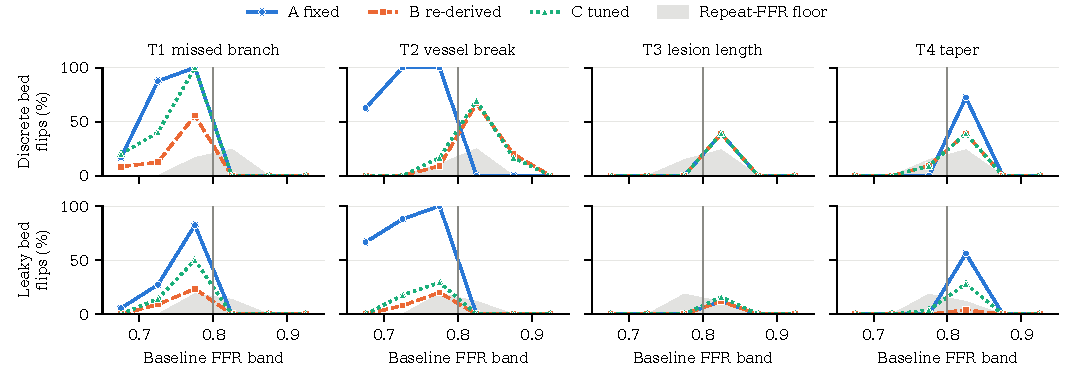
\includegraphics[width=\textwidth]{figures/fig2_flip_by_band.pdf}
\caption{Flip rate (proportion of models whose classification at FFR 0.80 changed) by baseline FFR band (0.05
wide, plotted at the band center; bands with fewer than three models omitted), error type, protocol (A--C) and bed
structure. The shaded area is the flip rate expected from repeat invasive FFR alone (standard deviation 0.018).}
\label{fig:band}
\end{figure*}

\subsection{Passes-and-Wrong Under Tuned Boundary Conditions}
Fitting one bed scaling to the clean territory flows (Protocol C) lowered the median perfusion residual of
topological-error models from 0.19 to 0.14 in the discrete bed and from 0.10 to 0.02 in the leaky bed, and reversed
more topological flips than it created relative to Protocol A (significant for leaky vessel breaks, $p < 0.001$).
Relative to Protocol B, it changed at most two topological-error decisions per cell ($p \geq 0.5$).
Protocol D matched the territory flows within 1\% in all but two models and corrected most of the topological error:
the median $|\Delta\mathrm{FFR}|$ of topological-error models fell to 0.005 in both beds, and their flip rate to 8\%
(discrete) and 6\% (leaky).

Tuning did not remove the error from every model (Fig.~\ref{fig:absorb}). After Protocol C, 20 of 104 topological-error
models (19\%, 13--28\%) in the discrete bed and 14 of 171 (8\%, 5--13\%) in the leaky bed passed the perfusion check
while their FFR was materially wrong (more than 0.05 from the clean value); after Protocol D, 21 of 104 (20\%,
14--29\%) and 9 of 171 (5\%, 3--10\%) did. Under Protocol B the proportions were 2\% and 6\%. Tuning raised them in
the discrete bed (McNemar $p < 0.001$ for C and D) but not in the leaky bed ($p \geq 0.12$). Under Protocol A they
were 12\% and 20\%. Models with
correct anatomy, tuned to perfusion measured with physiological noise, passed while materially wrong in 3.1\% (2.4--4.0\%) and 3.9\% (3.2--4.6\%) of draws, and their flip rates were 6.2\% and 7.2\%.
Looser thresholds of 13\% and 16\% raised the proportions (Supplementary Material).

Tuning also turned caliber errors into passes-and-wrong. With re-derived boundary conditions no caliber-error model
passed while materially wrong in either bed. After tuning, 5\% (C) and 18\% (D) did so in the discrete bed and 12\%
and 4\% in the leaky bed (McNemar against B, $p \leq 0.004$ in all four comparisons). Almost all were taper models
whose FFR tuning lowered: forcing the clean flow through a uniformly narrowed lumen raises its pressure drop
(Table~\ref{tab:results}).

\begin{figure}[!t]\centering
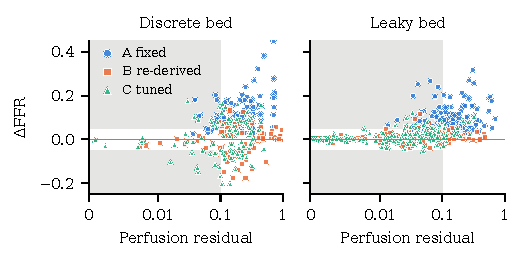
\includegraphics[width=\columnwidth]{figures/fig3_absorption.pdf}
\caption{Change in FFR against territory-perfusion residual for missed-branch and vessel-break models under Protocols A--C (Protocol D residuals lie below 0.01). Each point
is one model. The shaded areas hold models that pass the perfusion check (residual $< 0.10$) while materially wrong ($|\Delta\mathrm{FFR}| > 0.05$). The horizontal axis is linear below 0.01 and logarithmic above.}
\label{fig:absorb}
\end{figure}

\subsection{Side-Branch Loss Under Fixed and Tuned Resistance}
A missed side branch raised the computed FFR. In the 44 (discrete) and 71 (leaky) instances in which tuning was
defined, it raised FFR by a median of 0.095 and 0.047 with fixed boundary conditions. Protocol C reduced the shift to
0.077 and 0.015 (Wilcoxon signed-rank, $p < 0.001$ in both beds; Fig.~S3 in the Supplementary Material), and Protocol
D to 0.000 and 0.004, but 10 of 44 and 3 of 71 instances remained above 0.05 after Protocol D.

\subsection{Three-Dimensional Case Study}
The 3D case reproduced the reduced-order result. With the clean tree's resistances at the outlets, removal of the
side branch raised the 3D FFR at the measurement point from 0.870 to 0.944 ($\Delta$FFR $= +0.074$). With the clean
territory flows prescribed at the outlets (Protocol D), the same error changed FFR by $-0.0007$ (0.892 in both
geometries), so in this instance per-territory tuning removed the error. The reduced-order twins gave $+0.081$ and
$-0.0005$ for the same two conditions, and their baseline FFR was within 0.011 of the 3D values
(Fig.~\ref{fig:case3d}). In the cohort model of the same instance (discrete bed), the error gave $+0.127$ under
Protocol A and $-0.0007$ under Protocol D, whereas the single scaling of Protocol C left $+0.107$ with a residual of
0.30, which fails the check.
\begin{figure*}[!t]\centering
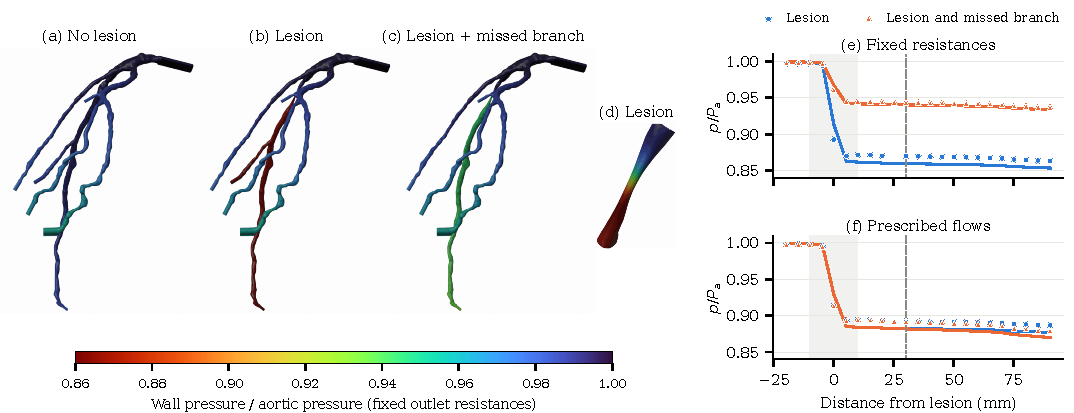
\includegraphics[width=\textwidth]{figures/fig5_case3d.pdf}
\caption{Three-dimensional case study (proximal LAD, 80\% DS). (a)--(c) Wall pressure relative to aortic pressure
with the clean tree's outlet resistances, without the lesion, with the lesion, and with the lesion and a missed side branch. The lesion lowers the downstream pressure (red); the missed branch raises it again (green), a shift
that would move a decision near 0.80. (d) Close-up of the lesion. (e), (f) Pressure along the artery with fixed
resistances and with prescribed clean territory flows. Markers show 3D cross-section averages and lines the reduced-order models on the meshed radius with the same outlet conditions. The shaded band is the lesion and the dashed line the measurement point.}
\label{fig:case3d}
\end{figure*} Two caveats apply. The meshed lumen was wider than the radius used by the reduced-order model (median
difference 0.14~mm; throat area-equivalent radius 0.276 against 0.231~mm), and on the requested radius the
reduced-order baseline was 0.761. A finer throat zone (12.5~\textmu m) changed the baseline FFR by at most 0.0021, against the error effect of 0.074
(Supplementary Material).

\subsection{Hyperemic Demand}\label{sec:demand}
With $k$ doubled and tripled, the stenosis sweep, cohort selection and all four protocols were repeated
(Supplementary Material). The median FFR of a 50\% DS lesion fell from 0.931 to 0.845 and 0.776, so the reselected
cohorts carried milder lesions, and fewer trees met the healthy-network criterion of the discrete bed (47 instances at
twice and 17 at three times the demand; the discrete arm is reported at twice the demand only). The directions held.
With fixed boundary conditions, topological errors changed 33--50\% of decisions against 1--5\% for caliber errors;
tuning reduced topological flips to 3--20\%; and after tuning, 3--20\% of topological-error and 1--14\% of
caliber-error models passed while materially wrong, against 0--5\% with re-derived boundary conditions.

% ---------------------------------------------------------------------------------------------------------------
\section{Discussion}
\subsection{What a Perfusion Check Shows After Tuning}
We asked whether a coronary flow model tuned to perfusion can still assign the wrong treatment. Three findings
answer this. First, with fixed boundary conditions the decision risk of segmentation lay mainly in the branching
structure of the lumen: a topological error changed the decision at 0.80 three to six times as often as a caliber
error of inter-observer magnitude, whose flip rates were of the order of repeat invasive measurement. This ranking
holds for the magnitudes studied, a whole branch or vessel segment against inter-observer caliber disagreement.

Second, how much of a topological error reaches the decision depends on the boundary conditions. Re-deriving or
tuning the bed reduced topological flips from 18--43\% to 2--20\% per error type, and the more flexible the tuning, the more of the
error it removed: per-territory tuning restored the flow that the missing branch had carried through the stenosis,
in the cohort and in the 3D case.

Third, after tuning the perfusion check no longer carried information about the error. A tuned model passes by
construction, whether its FFR has been corrected or not. In the discrete bed one in five tuned topological-error
models remained materially wrong under either form of tuning, and in both beds tuning produced passing models with
caliber errors that re-derived models did not, because restoring the clean flow through a narrowed lumen enlarges
its pressure drop. The check measured agreement with the fitted targets, not the correctness of the model.

Bed structure set the magnitude: in the leaky bed a deleted branch's conductance reappears as wall outflow at its
parent node, damping the error. Claims are therefore limited to directions that held in both; the
excess of passes-and-wrong over re-derived boundary conditions for topological errors held only in the discrete bed.

\subsection{Relation to Published Studies}
Published sensitivity analyses perturb lumen caliber at fixed branching, and comparisons of geometry with boundary
conditions rank them on a continuous output \cite{sankaran2016,tanade2022,korte2023}. Our results add that the
ranking depends on the error type and the boundary-condition protocol.

Two earlier findings that appeared to disagree are reproduced here. A side-branch effect of 13--15.5\% under fixed outlet resistance was reported in an idealized model and a model built from optical coherence tomography \cite{gamage2022}, whereas recalibrating a cohort-wide outlet resistance absorbed a large change in side-branch flow with little change in diagnostic accuracy \cite{gosling2020}. Both appear in our cohort, the first with fixed resistance and the second after re-derivation or tuning, so the difference follows
from the boundary-condition protocol.

Vessel breaks occur in the output of current segmentation methods despite high overlap scores \cite{bransby2026},
and a missing side branch removes few voxels, so the error types that carried the decision risk here are the ones that the usual overlap metrics do not measure, although topology-aware measures such as clDice
exist \cite{shit2021}.

\subsection{Implications and Practical Use}
Agreement with a fitted quantity does not by itself make a model credible, which also requires verification,
uncertainty quantification and applicability \cite{viceconti2025}. A missed branch that survived tuning raised FFR, biasing the decision toward
deferring treatment, whereas a tuned taper error lowered it, biasing the decision toward treatment.

For a user who computes FFR from an image, the results suggest four steps. First, check that the side branches
beyond the lesion are present and that no vessel ends early, because overlap scores do not reveal these errors.
Second, if the boundary conditions are tuned to perfusion, check the lumen caliber as well: diameter errors of
inter-observer size flipped decisions about as often as repeat invasive measurement without tuning, but produced
passing models with a wrong FFR after it. Third, record the perfusion mismatch before tuning; in the discrete bed
only 22\% of re-derived topological-error models passed, although in the leaky bed most did. Fourth, take most care near 0.80,
where decision changes concentrated. A developer can apply the same test to a pipeline and compare its rates with Table~\ref{tab:results}.
These steps follow from the results but are not validated decision rules.

\subsection{Limitations}
The inserted stenoses are idealized, and the reduced-order model is steady, without autoregulation or heart-rate
effects. The missed-branch and vessel-break magnitudes are design choices, and the caliber magnitudes come from
inter-observer statistics that likely overstate agreement. Protocols C and D were undefined for most right coronary
instances with a topological error, so their results for these errors describe the left coronary tree. Hyperemic
demand followed the segmented inlet radius and was below thermodilution values; at doubled and tripled demand,
fewer trees met the healthy-network criterion of the discrete bed. The 3D analysis covers one instance, with a
meshed lumen wider than the reduced-order radius; this offset shifts absolute FFR but not the paired differences on
which the findings rest. No invasive FFR was available, so the noise floor was modeled from published repeat
measurements.

\section{Conclusion}
In 150 controlled stenoses in 108 coronary trees, with fixed boundary conditions, topological segmentation errors
changed the decision at FFR 0.80 three to six times as often as caliber errors of inter-observer magnitude. Tuning the
boundary conditions to territory perfusion reduced these decision changes, and per-territory tuning removed most of
the error, as in a three-dimensional case. A tuned model, however, passes the perfusion check whether or not its FFR
is correct: after tuning, 5--20\% of topological-error and 4--18\% of caliber-error models passed while materially
wrong. A perfusion match after tuning is therefore not evidence of a correct FFR, and the segmentation must be checked
before tuning.

\section*{Data and Code Availability}
ImageCAS-X is available under CC BY 4.0 (doi:10.5281/zenodo.21887809). The code and the frozen cohort list are
available from the corresponding author on request.

\section*{Acknowledgment}
This work received no external funding, and the authors declare no conflicts of interest. The study used a public, anonymized dataset and required no ethics
approval.

\bibliographystyle{IEEEtran}
\bibliography{refs}

\end{document}
